\documentclass[12pt]{article}
\usepackage[utf8]{inputenc}
\usepackage{geometry}
\geometry{
	a4paper,
	left=20mm,
	right=20mm,
	top=25mm,
	bottom=20mm
}
\usepackage{amsmath}
\usepackage{amsfonts}
\usepackage{amssymb}
\usepackage{hyperref}
\hypersetup{
    colorlinks=true,
    linkcolor=black,
    filecolor=magenta,      
    urlcolor=blue,
    pdfpagemode=FullScreen,
    }
\usepackage{graphicx}
\graphicspath{ {./images/} }

\newcommand{\rmk}{$\surd$}
\newcommand{\sq}{$\square$}
\newcommand{\N}{\mathbb{N}}
\newcommand{\R}{\mathbb{R}}
\newcommand{\U}{\mathcal{U}}
\newcommand{\V}{\mathcal{V}}
\newcommand{\A}{\mathcal{A}}
\newcommand{\B}{\mathcal{B}}
\newcommand{\C}{\mathcal{C}}
\newcommand{\open}{\underset{open}{\subset}}
\newcommand{\closed}{\underset{closed}{\subset}}
\newcommand{\subsp}{\underset{subsp}{\subset}}
\newcommand{\seq}{\underset{seq}{\subset}}
\newcommand{\cl}{\overline}
\newcommand{\diff}{\,\backslash\,}
\newcommand{\exist}{\exists\,}
\newcommand{\homeo}{\underset{Homeo}{\simeq}}
\newcommand{\floor}[1]{\left\lfloor #1 \right\rfloor}

\begin{document}


\begin{titlepage}
	\begin{center}
		\vspace*{5cm}
		\textbf{\Large Mallow rank model Notes}
		\\	
		\vspace{1.5cm}
		\textbf{Taeyoung Chang}
		\vfill
		Article : Probabilistic Preference Learning with the Mallows Rank Model
        \\ Valeria Vitelli, \O{}ystein S\o{}rensen et al. 2018
		\\
		\vspace{0.8cm}
		Last Update : \today
		\vspace*{3cm}
		\thispagestyle{empty}
	\end{center}
\end{titlepage}

\clearpage
	
\section{Introduction}
\begin{itemize}
    \item Section 2 : Introduce the Bayesian Mallows model for rank data
    \item Section 2.1 : Discuss how the choice of the distance function influences the calculation of the partition function
    \item Section 2.2 : Deals with the choice of the prior distribution
    \item Section 2.3 \& 2.4 : Show how efficient Bayesian computation can be performed for this model, using a novel leap-and-shift proposal distribution.
    \item Section 3 : Develop and test an importance sampling scheme for computing the partition function, based on a pseudo-likelihood approximation of the Mallows model.
    \item Section 3.1 : Test and study the importance sampling estimation of the partition function
    \item Section 3.2 : Study the effect of this estimation on inference theoretically
    \item Section 3.3 : Study the effect of this estimation on inference by simulations
\end{itemize}
\section{A Bayesian Mallows model for complete rankings}
\begin{itemize}
    \item Setting : $n$ items and $N$ assessors. $\mathbf{R}_j\in \mathcal{P}_n$ denotes the ranking(the full set of ranks given to the $n$ items) of assessor $j$ for each $j=1,\cdots, N$. ($\mathcal{P}_n$ is a permutation set)
    \item $d(\cdot, \cdot): \mathcal{P}_n\times \mathcal{P}_n\rightarrow [0,\infty)$ is a distance function between two rankings.
    \begin{itemize}
        \item Kendall distance : number of pairs of distinct elements whose order in the two rankings are the opposite.
        \item Footrule distance : $\ell_1$ distance
        \item Spearman's distance : $\ell_2$ distance 
    \end{itemize}
    \item Mallows model is a class of non-uniform joint distributions for a ranking $\mathbf{r}$ on $\mathcal{P}_n$. $$P(\mathbf{r}|\alpha, \boldsymbol{\rho})=Z_n(\alpha, \boldsymbol{\rho})^{-1}\exp\{-\frac{\alpha}{n}d(\mathbf{r}, \boldsymbol{\rho})\}I(\mathbf{r}\in \mathcal{P}_n) $$
    \item $\boldsymbol{\rho}\in \mathcal{P}_n$ is the latent consensus ranking. $\alpha>0$ is a scale (or precision) parameter. \\i.e. $\alpha$ represents the level of agreement between assesssors, so that as $\alpha$ gets larger, ranking $\mathbf{r}$ aggregates more to $\boldsymbol{\rho}$ 
    \item $Z_n(\alpha, \boldsymbol{\rho})=\sum_{\mathbf{r}\in \mathcal{P}_n}e^{-\frac{\alpha}{n}d(\mathbf{r},\boldsymbol{\rho})}$ is the partition function.
    \item Assume that observed rankings $\mathbf{R}_1, \cdots, \mathbf{R}_N$ are conditionally independent given $\alpha$ and $\boldsymbol{\rho}$ and each of them is distributed according to the Mallows model with these parameters.
    \item Likelihood takes the form as \begin{equation}P(\mathbf{R}_1, \cdots, \mathbf{R}_N|\alpha, \boldsymbol{\rho})= Z_n(\alpha, \boldsymbol{\rho})^{-N}\exp\{-\frac{\alpha}{n}\sum_{j=1}^N d(\mathbf{R}_j, \boldsymbol{\rho})\}\prod_{j=1}^N I(\mathbf{R}_j\in \mathcal{P}_n) \end{equation}
    \item For large $n$, finding the MLE of $\boldsymbol{\rho}$ given fixed $\alpha$ is not feasible because the space of permutations $\mathcal{P}_n$ has $n!$ elements. 
\end{itemize}
\subsection{Distance Measures and Partition function}
\begin{itemize}
    \item For any right-invariant distance, it holds $d(\mathbf{r}_1, \mathbf{r}_2)=d(\mathbf{r}_1 \mathbf{r}_2^{-1}, \mathbf{1}_n)$ where $\mathbf{1}_n=\{1,2,\cdots,n\}$ and $\mathbf{r}_1 \mapsto \mathbf{r}_1 \mathbf{r}_2^{-1}$ is relabelling map. Note that a right-invariant distance is unaffected by a relabelling of the items.
    \item Partition function $Z_n(\alpha, \boldsymbol{\rho})$ does not depend on $\boldsymbol{{\rho}}$. 
    \begin{align*}
    \because Z_n(\alpha, \boldsymbol{\rho}) &= \sum_{\mathbf{r}\in \mathcal{P}_n}\exp\{-\frac{\alpha}{n}d(\mathbf{r},\boldsymbol{\rho})\} = \sum_{\mathbf{r}\in \mathcal{P}_n}\exp\{-\frac{\alpha}{n}d(\mathbf{r} \boldsymbol{\rho}^{-1}, \mathbf{1}_n)\}=\sum_{\mathbf{r'}\in \mathcal{P}_n}\exp\{-\frac{\alpha}{n}d(\mathbf{r'},\mathbf{1}_n)\} \\ Z_n(\alpha, \boldsymbol{\rho}) &= Z_n(\alpha)=\sum_{\mathbf{r}\in \mathcal{P}_n}\exp\{-\frac{\alpha}{n}d(\mathbf{r},\mathbf{1}_n)\}
    \end{align*}
    \item For some choice of right-invariant distance like Kendall distance, the partition function can be analytically computed. 
    \item But there are important and natural right-invariant distances for which the computation of the partition function is not feasible, such as the footrule distance and the Spearman's distance.
\end{itemize}
\subsection{Prior distributions}
\begin{itemize}
    \item Assume a priori that $\alpha$ and $\boldsymbol{\rho}$ are independent
    \item In this paper, the uniform prior $\pi(\boldsymbol{\rho})=\frac{1}{n!}I(\boldsymbol{\rho}\in \mathcal{P}_n)$ is employed.
    \item Also, for the scale parameter, this paper used a truncated exponential prior with density $\pi(\alpha | \lambda)=\lambda e^{-\lambda \alpha}I(\alpha\in [0, \alpha_{max}])/(1-e^{-\lambda \alpha_{max}})$ where the cut-off point $\alpha_{max}<\infty$ is large compared to the values supported by the data. In practice, in the computations involving the sampling of values for $\alpha$, truncation was never applied. We assign $\lambda$ a fixed value close to zero, implying a prior density for $\alpha$ which is quite flat.
\end{itemize}
\subsection{Inference}
\begin{itemize}
    \item The posterior distribution for $\boldsymbol{\rho}$ and $\alpha$ is given by
    \begin{equation}
        P(\boldsymbol{\rho}, \alpha| \mathbf{R}_1, \cdots, \mathbf{R}_N)\propto \frac{\pi(\boldsymbol{\rho})\pi(\alpha)}{Z_n(\alpha)^N} \exp \big\{-\frac{\alpha}{n}\sum_{j=1}^N d(\mathbf{R}_j, \boldsymbol{\rho})\big\}
    \end{equation}
    \item Note that marginal posterior mode of $\boldsymbol{\rho}$ from (2) does not depend on $\alpha$ and in case of uniform prior for $\boldsymbol{\rho}$, it coincides with the the MLE of $\boldsymbol{\rho}$ in (1). 
    \item The marginal posterior distribution of $\boldsymbol{\rho}$ is given by 
    \begin{equation}
        P(\boldsymbol{\rho} | \mathbf{R}_1, \cdots, \mathbf{R}_N)\propto \pi(\boldsymbol{\rho})\int_0^\infty \frac{\pi(\alpha)}{Z_n(\alpha)^N} \exp \big\{-\frac{\alpha}{n}\sum_{j=1}^N d(\mathbf{R}_j, \boldsymbol{\rho})\big\}\, d\alpha
    \end{equation}
    \item Note that for given data $\mathbf{R}=\{\mathbf{R}_1, \cdots, \mathbf{R}_N\},\quad  P(\boldsymbol{\rho} | \mathbf{R}_1, \cdots, \mathbf{R}_N)$ is determined \\ by $T(\boldsymbol{\rho}, \mathbf{R})=\sum_{j=1}^N d(\mathbf{R}_j, \boldsymbol{\rho})$
\end{itemize}
\subsection{Metropolis-Hastings Algorithm for Complete Rankings}
\begin{itemize}
    \item[\rmk] About the Metropolis-Hastings algorithm [ Hoff 2009 ]
    \begin{itemize}
        \item A general form of the Metropolis Hastings algorithm is as follows : \\ Target probability distribution is $p_0(x)$ for r.v. $X$. Given a current value $x^{(s)}$ of $X$, 
        \begin{enumerate}
            \item Generate $x^{*}$ from a proposal distribution $J_s(x^{*}|x^{(s)})$
            \item Compute the acceptance ratio $$ r=\frac{p_0(x^*)}{p_0(x^{(s)})}\, /\, \frac{J_s(x^*|x^{(s)})}{J_s(x^{(s)}|x^*)} = \frac{p_0(x^*)}{p_0(x^{(s)})}\frac{J_s(x^{(s)}|x^*)}{J_s(x^*|x^{(s)})} $$
            \item set $x^{(s+1)}$ to $x^*$ with probability $\min (1, r)$ \\ i.e. Sample $u\sim unif(0,1)$ and then if $u<r$ set $x^{(s+1)}=x^*$, else set $x^{(s+1)}=x^{(s)}$
        \end{enumerate}
        \item The proposal distribution $J_s$ may depend on the iteration number $s$
        \item The primary restriction placed on $J_s(x^*|x^{(s)})$ is that it does not depend on values in the sequence previous to $x^{(s)}$ so that the algorithm generates a Markov chain.
        \item Proposal distribution $J_s$ should be chosen to satisfy that the Markov chain is irreducible, aperiodic, and recurrent. 
        \item By Ergodic Thm, the empirical distribution of samples generated from such a Markov chain will converge to the stationary distribution( of the Markov chain), which agrees with the target distribution.
    \end{itemize}
    To obtain samples from the posterior in (2), we alternate between two steps.
    \begin{enumerate}
        \item Given $\alpha$ and $\boldsymbol{\rho}$, update $\boldsymbol{\rho}$ by proposing $\boldsymbol{\rho}'$
        \item Then, given $\alpha$ and $\boldsymbol{\rho}'$, update $\alpha$ by proposing $\alpha'$
    \end{enumerate}
    \item Updating $\boldsymbol{\rho}$ 
    \begin{itemize}
        \item Leap-and-Shift Proposal(L\&S)
        \begin{enumerate}
            \item Fix an integer $L\in \{1,2,\cdots, \floor{\frac{n-1}{2}}\}$
            \item Draw a random number $u\sim Unif\{1,2,\cdots, n\}$
            \item Define $\mathcal{S}\subset \{1,2,\cdots, n\}$ by $\mathcal{S}=\big[\max (1, \rho_u-L), \min (n, \rho_u+L)\big]\diff\{\rho_u\}$
            \item Draw a random number $r\sim Unif(\mathcal{S})$
            \item Let $\boldsymbol{\rho}^*\in \{1,2,\cdots, n\}^n$ have elements $\begin{cases}
            \rho_i^*=\rho_i & i\in \{1,2,\cdots,n\}\diff \{u\} \\\rho_u^*=r \end{cases}$\\ This step constitutes the leap step.
            \item Let $\Delta=\rho_u^*-\rho_u$. Note that $\Delta\neq 0$ 
            \item Define the proposed $\boldsymbol{\rho}'\in \mathcal{P}_n$ by below :
            \begin{enumerate}
                \item If $\Delta>0$ then $$\begin{cases}
                    \rho_u'=\rho_u^* \\ \rho_i'=\rho_i-1 & if \; \rho_u<\rho_i\leq \rho_u^* \\ \rho_i'=\rho_i & otherwise
                \end{cases} $$
                \item If $\Delta<0$ then $$\begin{cases}
                    \rho_u'=\rho_u^* \\ \rho_i'=\rho_i+1 & if \; \rho_u>\rho_i\geq \rho_u^* \\ \rho_i'=\rho_i & otherwise
                \end{cases} $$
            \end{enumerate} 
            This step constitutes the shift step.
        \end{enumerate}
        \item The probability mass function associated to the transition
        \begin{multline*}
            P_L(\boldsymbol{\rho}'|\boldsymbol{\rho}) = \sum_{u=1}^n P_L(\boldsymbol{\rho}'|U=u, \boldsymbol{\rho})P(U=u) \\ = \frac{1}{n}\sum_{u=1}^n\bigg\{I_{\{\boldsymbol{\rho}_{-u}\}}(\boldsymbol{\rho}_{-u}^*)I_{\{0<|\boldsymbol{\rho}_u-\boldsymbol{\rho}_u^*|\leq L\}}(\boldsymbol{\rho_u^*}) \Big[\frac{I_{\{L+1,\cdots, n-L\}}(\boldsymbol{\rho}_u)}{2L}+\sum_{z=1}^L \frac{I_{\{z\}}(\boldsymbol{\rho}_u)+I_{\{n-z+1\}}(\boldsymbol{\rho}_u)}{L+z-1} \Big]\bigg\} \\ +\; \frac{1}{n}\sum_{u=1}^n\bigg\{I_{\{\boldsymbol{\rho}_{-u}\}}(\boldsymbol{\rho}_{-u}^*)I_{\{|\boldsymbol{\rho}_u-\boldsymbol{\rho}_u^*|=1\}}(\boldsymbol{\rho_u^*}) \Big[\frac{I_{\{L+1,\cdots, n-L\}}(\boldsymbol{\rho}_u^*)}{2L}+\sum_{z=1}^L \frac{I_{\{z\}}(\boldsymbol{\rho}_u^*)+I_{\{n-z+1\}}(\boldsymbol{\rho}_u^*)}{L+z-1} \Big]\bigg\}
        \end{multline*}
        \item[\rmk] Interpretation for the equation above
        \begin{itemize}
            \item $ I_{\{\boldsymbol{\rho}_{-u}\}}(\boldsymbol{\rho_{-u}^*}) $ : indicator where given $u, \,\boldsymbol{\rho}_u$ and $\boldsymbol{\rho}'$, we can derive inverse transform $\boldsymbol{\rho}'\mapsto \boldsymbol{\rho}^*$ and then compare two sets $\boldsymbol{\rho}_{-u}$ and $\boldsymbol{\rho}_{-u}^*$
            \item $I_{\{0<|\boldsymbol{\rho}_u-\boldsymbol{\rho}_u^*|\leq L\}}(\boldsymbol{\rho}_u^*)$ : $\boldsymbol{\rho}_u^*=\boldsymbol{\rho}'_u$ and by construction of L\&S proposal, $\boldsymbol{\rho}_u^*\neq \boldsymbol{\rho}_u$ and $|\boldsymbol{\rho}_u^*-\boldsymbol{\rho}_u|\leq L$ should be satisfied. 
            \item If $\boldsymbol{\rho}_u\in \{L+1, \cdots, n-L\}$ then $\mathcal{S}=\big[\boldsymbol{\rho}_u-L, \boldsymbol{\rho}_u+L\big]\diff\{\boldsymbol{\rho}_u\}$, whose cardinality is $2L$. Hence, in this case the probability mass is $\frac{1}{2L}$. Else, if $\boldsymbol{\rho}_u\in \{1, \cdots, L\}$ then $\mathcal{S}=\big[1, \boldsymbol{\rho}_u+L\big]\diff\{\boldsymbol{\rho}_u\}$ whose cardinality is $\boldsymbol{\rho}_u+L-1$. Hence, in this case the probability mass is $\frac{1}{L+\boldsymbol{\rho}_u-1}$. Similar case is when $\boldsymbol{\rho}_u\in \{n-L+1, \cdots, n\}$ 
            \item The term added in the last line is for the special case where $ |\boldsymbol{\rho}_u-\boldsymbol{\rho}_u^*|=1$ holds.
        \end{itemize}
        \item[\sq] Simple representation for the transition probability
        \begin{itemize}
            \item As we calculate $P(\boldsymbol{\rho}'|\boldsymbol{\rho})$, we should consider two random draws
            \begin{itemize}
                \item Draw $u\sim Unif\{1,2,\cdots, n\}$
                \item For $S$ dependent on $\boldsymbol{\rho}_u$, draw $r\sim Unif(S)$
                \item The other works including shift step involve no randomness.
            \end{itemize}
            \item Simply put, $P(\boldsymbol{\rho}'|\boldsymbol{\rho})=\frac{1}{n}\cdot\frac{1}{|S|}$ for many cases.
            \item However, if $|\boldsymbol{\rho}_u'-\boldsymbol{\rho}_u|=1$ then we should consider something more. 
            \item When $|\boldsymbol{\rho}_u'-\boldsymbol{\rho}_u|>1$ then $u$ is the only possible index that proposes $\boldsymbol{\rho}'$ from $\boldsymbol{\rho}$. On the other hand, when $|\boldsymbol{\rho}_u'-\boldsymbol{\rho}_u|=1$, there must be only one index $u'$ other than $u$ s.t. $|\boldsymbol{\rho}_{u'}'-\boldsymbol{\rho}_{u'}|=1$ so that $u'$ can also proposes $\boldsymbol{\rho}'$ from $\boldsymbol{\rho}$.
            \item In this special case, $P(\boldsymbol{\rho}'|\boldsymbol{\rho})=\frac{1}{n}\cdot\frac{1}{|S|}+\frac{1}{n}\cdot\frac{1}{|S'|}$ where $S$ is produced from drawing $u$ and $S'$ is produced from drawing $u'$
            \item Using this logic, we can rewrite the equality about $P_L(\boldsymbol{\rho}'|\boldsymbol{\rho})$ as the following 
            \begin{align*}
                P_L(\boldsymbol{\rho}'|\boldsymbol{\rho}) &= \sum_{u=1}^n P_L(\boldsymbol{\rho}'|U=u, \boldsymbol{\rho})P(U=u) \\ &= \frac{1}{n}\sum_{u=1}^n I(\boldsymbol{\rho}', \boldsymbol{\rho}, u) \frac{1}{|S^{(u)}|}
            \end{align*}
            where $I(\boldsymbol{\rho}', \boldsymbol{\rho}, u)$ is an indicator for possibility of proposal from $\boldsymbol{\rho}$ to $\boldsymbol{\rho}'$ given $u$ is drawed and $S^{(u)}$ is the set $S$ given $u$ is drawed \\ If $\boldsymbol{\rho}'$ is proposed from $\boldsymbol{\rho}$ then typically $I(\boldsymbol{\rho}', \boldsymbol{\rho}, u)=1$ for only one $u$ but if $|\boldsymbol{\rho}_u'-\boldsymbol{\rho}_u|=1$ then $I(\boldsymbol{\rho}', \boldsymbol{\rho}, u')=1$ also holds for another $u'$ different from $u$ 
        \end{itemize} 
        \item The acceptance probability when updating $\boldsymbol{\rho}$ is 
        $\min\{1, r\}$ where $r$ is given as 
        \begin{align*}
            r &=\frac{P(\boldsymbol{\rho}', \alpha | \mathbf{R})}{P(\boldsymbol{\rho}, \alpha | \mathbf{R})}\cdot \frac{P_L(\boldsymbol{\rho}|\boldsymbol{\rho}')}{P_L(\boldsymbol{\rho}'|\boldsymbol{\rho})} \\ &= \frac{P_L(\boldsymbol{\rho}|\boldsymbol{\rho}')}{P_L(\boldsymbol{\rho}'|\boldsymbol{\rho})} \cdot \frac{\pi(\boldsymbol{\rho}')}{\pi(\boldsymbol{\rho})}\exp\big\{-\frac{\alpha}{n}\sum_{j=1}^N \big[d(\mathbf{R}_j, \boldsymbol{\rho}')-d(\mathbf{R}_j, \boldsymbol{\rho})\big] \big\}
        \end{align*} 
        \item[\rmk] The term $\sum_{j=1}^N \big[d(\mathbf{R}_j, \boldsymbol{\rho}')-d(\mathbf{R}_j, \boldsymbol{\rho})\big]$ above can be computed efficiently since most elements of $\boldsymbol{\rho}$ and $\boldsymbol{\rho}'$ are equal and we can put aside indices $i$ s.t. $\rho_i=\rho'_i$
        \item $L$ is a tuning parameter for MCMC algorithm.  
    \end{itemize}
    \item Updating $\alpha$
    \begin{itemize}
        \item Sample a proposal $\alpha '$ from a lognormal distribution $\log\mathcal{N}(\log(\alpha), \sigma_\alpha^2)$
        \item[\rmk]  Note that $X\sim \log\mathcal{N}(\mu, \sigma^2)\Leftrightarrow Y=\log X\sim N(\mu, \sigma^2)$. The pdf of $X\sim \log\mathcal{N}(\log(\mu), \sigma^2)$ is written as $f(x ; \mu, \sigma)=\frac{1}{\sqrt{2\pi \sigma^2}}\exp\bigl(-\frac{1}{2\sigma^2}(\log x -\log \mu)^2 \bigr)\frac{1}{x}\,I(x>0)$
        \item The probability density function associated to the transition is $$J(\alpha'|\alpha)=\frac{1}{\sqrt{2\pi \sigma_\alpha^2}}\exp\bigl(-\frac{1}{2\sigma_\alpha^2}(\log \alpha' -\log \alpha)^2 \bigr)\frac{1}{\alpha'}$$
        Accordingly, we have the ratio $\frac{J(\alpha'|\alpha)}{J(\alpha|\alpha')}=\frac{\alpha}{\alpha'}$ 
        \item Acceptance probability is $\min\{1, r\}$ where $r$  is given as 
        \begin{align*}
            r &= \frac{P(\boldsymbol{\rho}, \alpha' | \mathbf{R})}{P(\boldsymbol{\rho}, \alpha | \mathbf{R})} \,/\, \frac{J(\alpha'|\alpha)}{J(\alpha|\alpha')} \\ &= \frac{\alpha'}{\alpha}\frac{\pi(\alpha')}{\pi(\alpha)}\frac{Z_n(\alpha)^N}{Z_n(\alpha')^N}\exp \big\{-\frac{\alpha'-\alpha}{n}\sum_{j=1}^N d(\mathbf{R}_j, \boldsymbol{\rho})\big\}
        \end{align*}
        \item $\sigma_\alpha^2$ is a tuning parameter for MCMC algorithm. Additional parameter $\alpha_{jump}$ can be used to update $\alpha$ only every $\alpha_{jump}$ updates of $\boldsymbol{\rho}$
    \end{itemize}
\end{itemize}
\section{Approximating the Partition Function $Z_n(\alpha)$ via \\Off-line Importance Sampling}
\begin{itemize}
    \item The partition function $Z_n(\alpha)$ is available in close form for Kendall's, Hamming, and Cayley distances.
    \item But this is not the case for footrule and Spearman distances.
    \item To handle these cases, we propose an approximation of the partition function $Z_n(\alpha)$ based on importance sampling. 
    \item Recall that given right-invarant distances, the partition function does not depend on $\boldsymbol{\rho}$. 
    \item Obtain an off-line approximation of the partition function on a gird of $\alpha$ values. 
    \begin{itemize}
        \item In computer science, an online algorithm is one that can process its input piece-by-piece in a serial fashion, i.e. in the order that the input is fed to the algorithm, without having the entire input available from the start.
        \item In contrast, an offline algorithm is given the whole problem data from the beginning and is required to output an answer which solves the problem at hand. 
    \end{itemize}
    \item Then interpolate it to yield an estimate of $Z_n(\alpha)$ over a continuous range and read off needed values to compute the acceptance probabilities rapidly.
    \item Estimate the partition function directly using Importance Sampling (IS) approach
    \begin{itemize}
        \item For $K$ rank vectors $\mathbf{R}^1,\cdots, \mathbf{R}^K$ sampled from an IS auxiliary distributution $q(\mathbf{R})$, the unbiased IS estimate of $Z_n(\alpha)$ is given by \begin{equation}
            \hat{Z}_n(\alpha)=\frac{1}{K}\sum_{k=1}^K \exp\big\{-\frac{\alpha}{n}d(\mathbf{R}^k, \mathbf{1}_n) \big\}\frac{1}{q(\mathbf{R}^k)}
        \end{equation} 
        \item Importance sampling
        \begin{itemize}
            \item Suppose our goal is estimate $\mu=E_p[f(X)]$ i.e. the expected value of $f(X)$ under $X\sim p$
            \item For a probability density $q$ other than $p$, we can calculate that $$\mu=E_p[f(X)]=\int f(x)p(x)\, dx=\int \frac{f(x)p(x)}{q(x)}q(x)\,dx=E_q\Big[\frac{f(X)p(X)}{q(X)}\Big] $$ 
            i.e. $\mu$ equals the expected value of $\frac{f(X)p(X)}{q(X)}$ under $X\sim q$
            \item The importance sampling estimate of $\mu$ is $$\hat \mu_q =\frac{1}{K}\sum_{k=1}^K \frac{f(X_i)p(X_i)}{q(X_i)} \quad \; where \; X_i\sim q$$
            \item The basic idea of importance sampling is to sample the states from a different distribution to lower the variance of estimation of $\mu$ or when sampling from original density $p$ is difficult.
            \item Reference : Wikipedia and \href{https://statweb.stanford.edu/~owen/mc/Ch-var-is.pdf}{Lecture note from standford.edu}
        \end{itemize}
        \item IS estimate of $Z_n(\alpha)$ in (4) is derived as the following
        \begin{align*}
            Z_n(\alpha)&=\sum_{\mathbf{R}\in \mathcal{P}_n}\exp\{-\frac{\alpha}{n}d(\mathbf{R},\mathbf{1}_n)\} =\sum_{\mathbf{R}\in \mathcal{P}_n}\frac{1}{P(\mathbf{R})}\exp\{-\frac{\alpha}{n}d(\mathbf{R},\mathbf{1}_n)\}P(\mathbf{R}) \\ &=E_{R\sim P(R)}\Big[ \frac{1}{P(\mathbf{R})}\exp\{-\frac{\alpha}{n}d(\mathbf{R},\mathbf{1}_n)\}\Big] = E_{R\sim P(R)}\big[f(\mathbf{R}) \big]
        \end{align*}
        where $f(\mathbf{R})=\frac{1}{P(\mathbf{R})}\exp\{-\frac{\alpha}{n}d(\mathbf{R},\mathbf{1}_n)\}$ and $P(\mathbf{R})$ is abbreviation of $P(\mathbf{R}|\alpha, \mathbf{1}_n)$
        \begin{equation*}
            \hat{Z}_n(\alpha)=\frac{1}{K}\sum_{k=1}^K \frac{f(\mathbf{R}^k)P(\mathbf{R}^k)}{q(\mathbf{R}^k)} =\frac{1}{K}\sum_{k=1}^K \exp\big\{-\frac{\alpha}{n}d(\mathbf{R}^k, \mathbf{1}_n) \big\}\frac{1}{q(\mathbf{R}^k)}\quad where \;\, \mathbf{R}^k\sim q(\mathbf{R})
        \end{equation*}
        \item While we cannot sample $\mathbf{R}$ from $P(\mathbf{R}|\alpha, \mathbf{1}_n)$ ($\because$ we don't know the value of $Z_n(\alpha)$) it must be computationally feasible to sample $\mathbf{R}$ from $q(\mathbf{R})$.
        \item The more $q(\mathbf{R})$ resembles the Mallows likelihood $P(\mathbf{R}^k | \alpha, \mathbf{1}_n)$, the smaller is the variance of $\hat{Z}_n(\alpha)$. 
        \item We shall use the following psuedo-likelihood approximation for $q(\mathbf{R})$
        \begin{enumerate}
            \item Sample $(i_1, \cdots, i_n)\in \mathcal{P}_n$, which gives the order of the psuedo-lieklihood factorization.
            \item Factorization is given as \begin{equation*}
                P(\mathbf{R}|\mathbf{1}_n)=P(R_{i_n}|\mathbf{1}_n)P(R_{i_{n-1}}|R_{i_n}, \mathbf{1}_n)\cdots P(R_{i_2}|R_{i_3}, \cdots, R_{i_n}, \mathbf{1}_n)P(R_{i_1}|R_{i_2}, \cdots, R_{i_n}, \mathbf{1}_n)
            \end{equation*}
            
            \item The conditional distributions are given by
            \begin{figure}[h]
                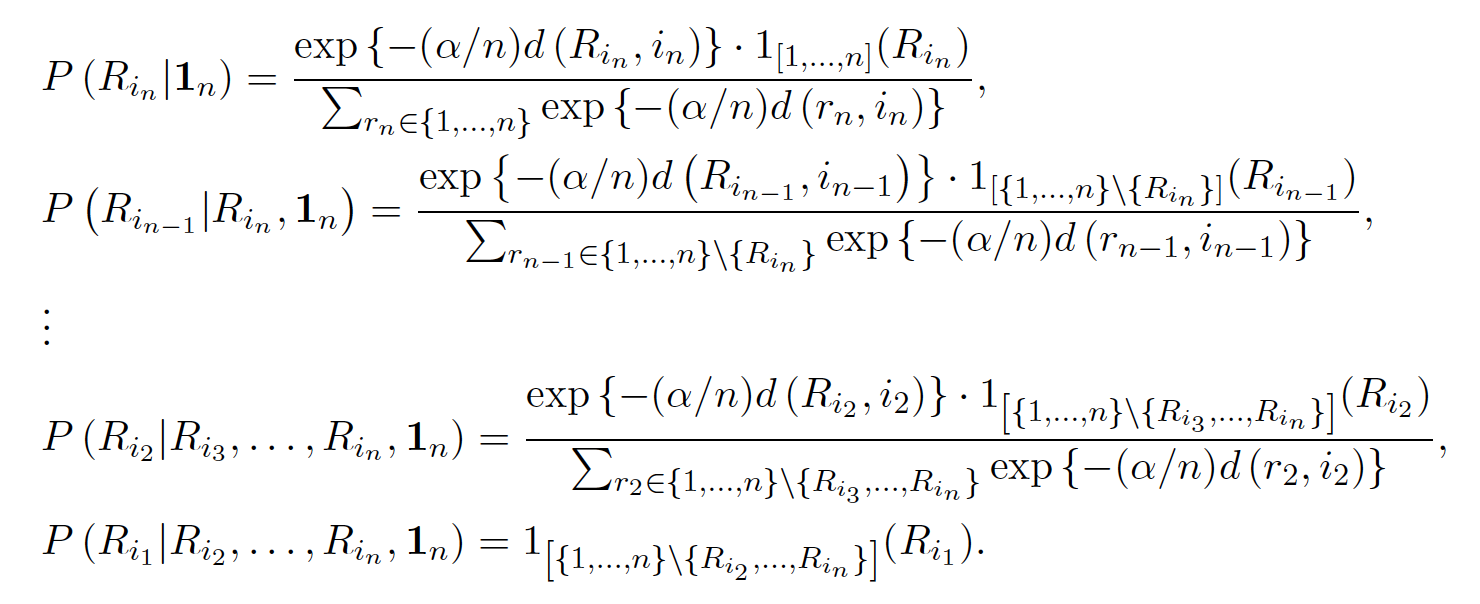
\includegraphics[width=15cm]{ConDist}
                \centering
            \end{figure}
            \\ Each factor is a simple univariate distribution. 
            \item For given value of $\alpha$, sample $R_{i_n}$ first, and then conditionally on that, $R_{i_{n-1}}$ and so on. The $k$-th full sample $\mathbf{R}^k$ has probability \begin{equation*}
                q(\mathbf{R}^k)=P(R_{i_n}^k|\mathbf{1}_n)P(R_{i_{n-1}}^k|R_{i_n}^k, \mathbf{1}_n)\cdots P(R_{i_2}^k|R_{i_3}^k, \cdots, R_{i_n}^k, \mathbf{1}_n)
            \end{equation*}       
        \end{enumerate}
        \item Keeping the psuedo-likelihood with the same distance as the one in the target was most accurate and efficient so we shall use the distance in (4) as same as the distance in (2).
    \end{itemize}
\end{itemize}
\subsection{Testing the Importance Sampler}
\begin{itemize}
    \item Over a discrete grid of 100 equally spaced $\alpha$ values between 0.01 and 10(this is the range of $\alpha$ which turned out to be relevant in all our applications, typically $\alpha<5$), we produce a smooth partition function simply using a polynomial of degree 10.
    \item[\rmk] What we have is 100 data points of $(\alpha^{(i)}, \hat Z_n(\alpha^{(i)}))$'s. A smooth partition function is produced by fitting multiple linear regression for the model $$\log \hat Z_n(\alpha)=\beta_0+\beta_1 \alpha+\beta_2 \alpha^2+\cdots+\beta_{10} \alpha^{10}$$ so that only thing we should store before implementing MCMC for the partition function is those estimated beta parameter values.
    \item As $K$ goes large, $\hat{Z}_n$ becomes precise estimates for $Z_n$.  
\end{itemize}
\subsection{Effect of $\hat{Z}_n$ on the MCMC}
\begin{itemize}
    \item Theoretical results regarding the convergence of the MCMC, when using the IS approximation of the partition function.
    \item Algorithm using $\hat{Z}_n$ instead of $Z_n$ converges to the posterior distribution proportional to \begin{equation} \frac{1}{\hat{C}(\mathbf{R})}\frac{\pi(\boldsymbol{\rho})\pi(\alpha)}{\hat{Z}_n(\alpha)^N} \exp \big\{-\frac{\alpha}{n}\sum_{j=1}^N d(\mathbf{R}_j, \boldsymbol{\rho})\big\} \end{equation} where the normalizing factor $\hat{C}(\mathbf{R})=\int\sum_{\boldsymbol{\rho}\in \mathcal{P}_n}\frac{\pi(\boldsymbol{\rho})\pi(\alpha)}{\hat{Z}_n(\alpha)^N} \exp \big\{-\frac{\alpha}{n}\sum_{j=1}^N d(\mathbf{R}_j, \boldsymbol{\rho})\big\}\, d\alpha $
    \item The approximate posterior (5) converges to the correct posterior (2), if $K$ increases with $N$, $K=K(N)$ and $$\lim_{N \to \infty}(\frac{\hat{Z}_n^{K(N)}(\alpha)}{Z_n(\alpha)})^N =1 \quad \forall \; \alpha$$
    \item For this, it is sufficient that $K(N)$ grows faster than $c\cdot N^2$ where $c$ depends on $\alpha, n, d( \;,\; )$ 
\end{itemize}
\subsection{Testing Approximations of the MCMC in Inference}
\begin{itemize}
    \item The main positive result from the perspective of practical applications was \begin{enumerate}
        \item The relative lack of sensitivity of the posterior inferences to the specification of the prior for the scale parameter $\alpha$
        \item The apparent robustness of the marginal posterior inferences on $\boldsymbol{\rho}$ on the choice of the approximation of the partition function $Z_n(\alpha)$.
    \end{enumerate}
\end{itemize}
\section{Extensions to Partial Rankings and Heterogeneous \\ Assessor Pool}
\begin{itemize}
    \item We will relax two assumptions of the previous sections.
    \begin{enumerate}
        \item Each assessor ranks all $n$ items. 
        \item The assessors are homogeneous, all sharing a common consensus ranking.
    \end{enumerate}
\end{itemize}
\subsection{Ranking of the Top Ranked Items}
\begin{itemize}
    \item Often only a subset of the items is ranked.
    \item These situations can be handled conveninetly in Bayesian framework by applying data augmentation techniques.
    \item We shall consider the case of the top-$k$ ranks.
    \item Setting 
    \begin{itemize}
        \item Among $n$ items $\{A_1, \cdots, A_n\}$, each assessor $j$ has ranked the subset of items $\mathcal{A}_j\subset\{A_1, \cdots, A_n\}$ giving them top ranks from $1$ to $n_j=|\mathcal{A}_j|$. 
        \item Before, we had complete ranking $\mathbf{R}_j\in \mathcal{P}_n$, but now, we denote $\mathbf{R}_j$ as partial ranking.
        \item We have augemented ranking vectors $\tilde{\mathbf{R}}_j\in \mathcal{P}_n$ where unknown part follows a symmetric prior on the permutations of $(n_j+1, \cdots, n)$ for each $j=1, \cdots, N$
    \end{itemize}
    \item MCMC algorithm
    \begin{itemize}
        \item $\mathcal{S}_j$ : set of all possible augmented random vectors given original partially ranked items together with the allowable `fill-ins' of the missing ranks, for each $j=1, \cdots, N$
        \item Our goal is to sample from the posterior distribution \begin{equation*}
            P(\alpha, \boldsymbol{\rho}\, |\, \mathbf{R}_1, \cdots, \mathbf{R}_N)=\sum_{\tilde{\mathbf{R}}_1\in \mathcal{S}_1}\cdots \sum_{\tilde{\mathbf{R}}_N\in \mathcal{S}_N}P(\alpha, \boldsymbol{\rho}, \tilde{\mathbf{R}}_1, \cdots,\tilde{\mathbf{R}}_N\, |\, \mathbf{R}_1, \cdots, \mathbf{R}_N )
        \end{equation*}
        \item Our MCMC algorithm alternates between
        \begin{enumerate}
            \item  sampling the augmented ranks given the current values of $\alpha$ and $\boldsymbol{\rho}$
            \item sampling $\alpha$ and $\boldsymbol{\rho}$ given the current values of the augmented ranks.
        \end{enumerate}
        \item The latter is done similar as in Section 2.4, where in this case $\mathbf{R}_1, \cdots, \mathbf{R}_N$ is replaced by $\tilde{\mathbf{R}}_1, \cdots,\tilde{\mathbf{R}}_N$ 
        \item For the former, given the current $\tilde{\mathbf{R}}_j$ (which embeds info contained in $\mathbf{R}_j$) and the current values of $\alpha$ and $\boldsymbol{\rho}$, $\tilde{\mathbf{R}}_j'$ is sampled in $\mathcal{S}_j$ from a uniform proposal distribution which is obviously symmetric.
        \\ The proposed $\tilde{\mathbf{R}}_j'$ is accepted with probability $\min\{1,r\}$ with \begin{align*}
            r&= \frac{P(\tilde{\mathbf{R}}_1, \cdots, \tilde{\mathbf{R}}_j',\cdots, \tilde{\mathbf{R}}_N\,|\, \alpha, \boldsymbol{\rho})}{P(\tilde{\mathbf{R}}_1, \cdots, \tilde{\mathbf{R}}_j,\cdots, \tilde{\mathbf{R}}_N\,|\, \alpha, \boldsymbol{\rho})} \\ &=\exp[-\frac{\alpha}{n}\big\{d(\tilde{\mathbf{R}}_j', \boldsymbol{\rho})-d(\tilde{\mathbf{R}}_j, \boldsymbol{\rho}) \big\}] \end{align*}
    \end{itemize}
    \item Note that we can generalize this algorithm to generic partial ranking, where items partially ranked by each assessor are not necessarily the top ranked items. 
\end{itemize}
\subsubsection{Effects of Unranked Items on the Top-$k$ Consensus Ranking}
\begin{itemize}
    \item It is possible that the number of items is large and  there are items which none of the assessors included in their top-list. Can we ignore such `left-over' items and consider only the items explicitly ranked by at least one assessor?
    \item The two main points are that
    \begin{itemize}
        \item Only items explicitly ranked by the assessors appear in top positions of the consesnsus ranking.
        \item When considering the MAP(maximum a posteriori) consensus ranking, excluding the left-over items from the ranking procedure already at the start has no effect on how the remaining ones will appear in such consensus ranking.
    \end{itemize}
    \begin{figure}[h]
        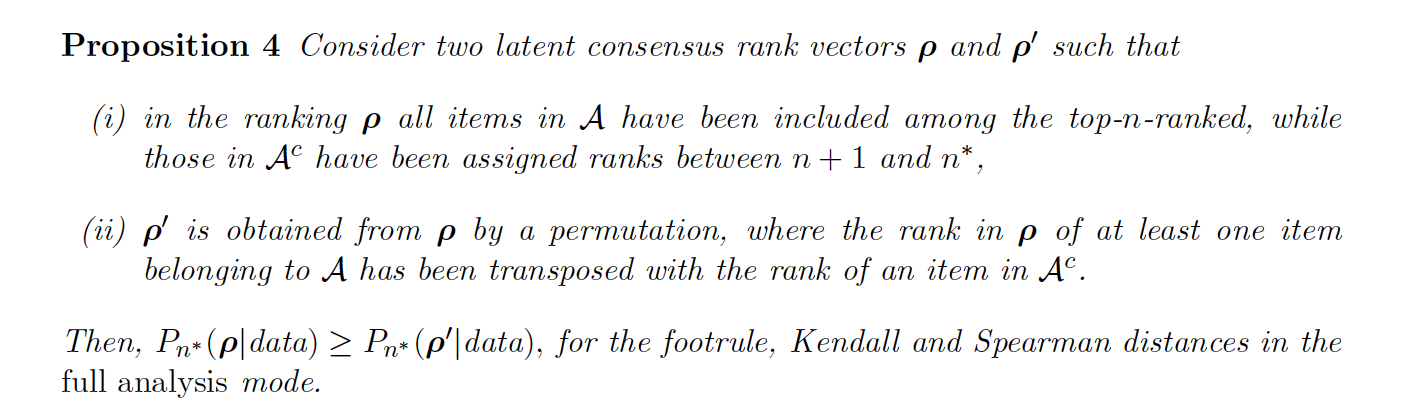
\includegraphics[width=\textwidth]{Proposition4.png}
        \centering
    \end{figure}
    \item[\rmk] The above proposition says that the MAP estimate for consensus ranking assigns $n$ highest ranks to explicitly ranked items in the data (Note that here we denote the number of total items as $n^*$)
    \begin{figure}[h]
        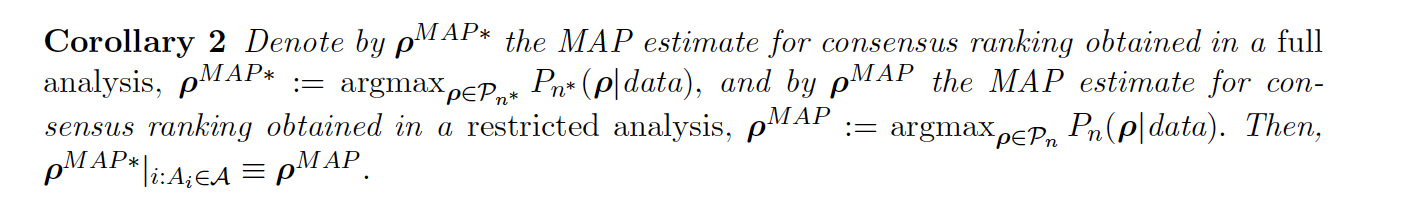
\includegraphics[width=\textwidth]{Corollary2.png}
        \centering
    \end{figure}
    \item[\rmk] Note that full analysis, which includes the complete set of all  items, cannot always be carried out in practice due to the fact that left-over items might be unknown or too many for realistic computation. The corollary guarantees that the top-$n$ items in the MAP consensus ranking do not depend on whether we include left-over items in the analysis. 
\end{itemize}
\subsection{Pairwise Comparison}
\begin{itemize}
    \item Often, assessors compare pairs of items rather than ranking all or a subset of items. 
    \item Notation for pairwise comparison 
    \begin{itemize}
        \item $A_r\prec A_s$ : $A_s$ is preferred to $A_r$, so that $A_s$ has a lower rank than $A_r$ 
        \item $\mathcal{B}_j$ : pairwise orderings or preferences stated by assessor $j$
        \item $\mathcal{A}_j$ : set of items constrained by asessor $j$
        \item $tc(\mathcal{B}_j)$ : the transitive closure of $\mathcal{B}_j$, containing all pairwise orderings of the elements in $\mathcal{A}_j$ induced by $\mathcal{B}_j$.
    \end{itemize} 
    \item[(Ex)] $\mathcal{B}_j=\{A_1\prec A_2, A_2\prec A_5\} \Rightarrow tc(\mathcal{B}_j)=\{A_1\prec A_2, A_2\prec A_5, A_1\prec A_5\} \\ \mathcal{B}_k=\{A_1\prec A_2, A_2\prec A_5, A_4\prec A_5\} \Rightarrow tc(\mathcal{B}_k)=\{A_1\prec A_2, A_2\prec A_5, A_1\prec A_5, A_4\prec A_5\}$
    \item In the MCMC algorithm, we need to propose augmented ranks which obey the partial ordering constraints given by each assessor, to avoid a large number of rejections, with the difficulty that none of the items is now fixed to a given rank.
    \item We can also handle the case when assessors give ties : in such a situation, each pair of items resulting in a ties is randomized to a preference at each data augmentation step inside the MCMC.
    \item The main idea of MCMC algorithm remains the same as in the Section 4.1
    \item The difference is that here, a `modified' leap-and-shift proposal distribution, rather than a uniform proposal distribution, is used to sample augmented ranks.
    \item `Modified' Leap-and-Shift proposal \\ Given a full augmented rank vector $\tilde{\mathbf{R}}_j$ compatible with $tc(\mathcal{B}_j)$, we shall propose $\tilde{\mathbf{R}}_j'$
        \begin{enumerate}
            \item Draw a random number $u\sim Unif\{1,2,\cdots, n\}$
            \item If $A_u \notin \mathcal{A}_j$ then complete the leap step by drawing $\tilde{R}_{uj}^*\sim Unif\{1,2,\cdots, n\}$
            \item If $A_u \in \mathcal{A}_j$ then complete the leap step by drawing $\tilde{R}_{uj}^*\sim Unif\{l_j+1, \cdots, r_j-1\}$ where $l_j$ and $r_j$ are defined by
            \begin{itemize}
                \item $l_j=\max\{\tilde{R}_{kj} : A_k\in \mathcal{A}_j, k\neq u, (A_k\succ A_u)\in tc(\mathcal{B}_j) \}$ with convention that $l_j=0$ if the set is empty
                \item $r_j=\min\{\tilde{R}_{kj} : A_k\in \mathcal{A}_j, k\neq u, (A_k\prec A_u)\in tc(\mathcal{B}_j) \}$ with convention that $r_j=n+1$ if the set is empty
                \item[\rmk] Briefly, $l_j$ is given rank of the item whose rank is closest to $A_u$ among all assessed items preferred to $A_u$, and $r_j$ is given rank of the item whose rank is closest to $A_u$ among all assessed items less preferred than $A_u$.
            \end{itemize} 
             This step constitutes the leap step.
            \item Let $\Delta=\tilde{R}_{uj}^*-\tilde{R}_{uj}$. 
            \item Define the proposed $\tilde{\mathbf{R}}_j'$ by below :
            \begin{enumerate}
                \item If $\Delta>0$ then $$\begin{cases}
                    \tilde{R}_{uj}'=\tilde{R}_{uj}^* \\ \tilde{R}_{ij}'=\tilde{R}_{ij}-1 & if \; \tilde{R}_{uj}<\tilde{R}_{ij}\leq \tilde{R}_{uj}^* \\ \tilde{R}_{ij}'=\tilde{R}_{ij} & otherwise
                \end{cases} $$
                \item If $\Delta<0$ then $$\begin{cases}
                    \tilde{R}_{uj}'=\tilde{R}_{uj}^* \\ \tilde{R}_{ij}'=\tilde{R}_{ij}+1 & if \; \tilde{R}_{uj}>\tilde{R}_{ij}\geq \tilde{R}_{uj}^* \\ \tilde{R}_{ij}'=\tilde{R}_{ij} & otherwise
                \end{cases} $$
                \item If $\Delta=0$ then $\tilde{\mathbf{R}_j'}=\tilde{\mathbf{R}_j}$
            \end{enumerate} 
            This step constitutes the shift step. (In fact the shift step remains unchanged from the original one.)
        \end{enumerate}
    \item Note that this modified leap-and-shift is symmetric proposal. Hence we use the same acceptance probability as in Section 4.1
\end{itemize}
\subsection{Clustering Assessors based on their Rankings of All Items}
\begin{itemize}
    \item So far we have assumed that there exists a unique consensus ranking shared by all assessors. 
    \item The possibility of dividing assessors into more homogeneous subsets, each sharing a consesnsus ranking of the items, brings the model closer to reality. 
    \item We introduce a mixture of Mallows models to handle heterogeneity.
    \begin{itemize}
        \item Assume that the data consist of complete rankings.
        \item $z_j\in \{1,\cdots, C\}$ assigns assessor $j$ to one of $C$ clusters, for each $j=1,\cdots, N$ \\ i.e. $z_1, \cdots, z_N$ are cluster labels.
        \item The assessments $\mathbf{R}$ within each cluster $c\in\{1,\cdots, C\}$ are described by a Mallows model with parameters $\alpha_c$ and $\boldsymbol{\rho}_c$ which is the cluster consensus. 
        \item Assume conditional independence across the clusters.
        \item Likelihood for the observed rankings $\mathbf{R}_1, \cdots, \mathbf{R}_N$ is given by \begin{equation*}
            P(\mathbf{R}_1, \cdots, \mathbf{R}_N|\{\alpha_c, \boldsymbol{\rho}_c\}_{c=1,\cdots, C}, z_1, \cdots, z_N)= \prod_{j=1}^N \frac{1}{Z_n(\alpha_{z_j})}\exp\{-\frac{\alpha_{z_j}}{n} d(\mathbf{R}_j, \boldsymbol{\rho}_{z_j})\}
        \end{equation*}
        \item Assumption for priors
        \begin{enumerate}
            \item $\boldsymbol{\rho}_1, \cdots \boldsymbol{\rho}_C \overset{indep}{\sim} \pi_{\boldsymbol{\rho}}$ where $\pi_{\boldsymbol{\rho}}$ is a uniform prior on $\mathcal{P}_n$ as before.
            \item $\alpha_1, \cdots, \alpha_C \overset{indep}{\sim} \pi_\alpha$ where $\pi_\alpha$ is a truncated exponential prior with shared $\lambda$
            \item $\tau_c$ is the probability that an assessor belongs to the c-th cluster. \\ $\tau_c\geq 0 \quad \forall c=1,\cdots, C$ and $\sum_{c=1}^C \tau_c=1$. \; $(\tau_1, \cdots \tau_C)$ are assigned the standard symmetric Dirichlet prior $\mathcal{D}(\psi, \cdots, \psi)$
            \item $P(z_j=c \,|\, \tau_1, \cdots, \tau_C)=\tau_c \quad \forall c=1,\cdots C$ and $z_1, \cdots z_N$ are conditionally i.i.d.
        \end{enumerate}
    \end{itemize}
    \item The number of clusters $C$ is often not known, and the selection of $C$ can be based on different criteria.
    \begin{itemize}
        \item Here we use the posterior distribution of the within-cluster sum of distances of the observed ranks from the corresponding cluster consensus.
        \item We expect to observe an `elbow' in the within-cluster distance posterior distribution as a function of $C$, identifying the optimal number of clusters. \\ (cf. Figure 6 in Section 4.4 )
    \end{itemize}
    \item MCMC algorithm
    \begin{itemize}
        \item The algorithm alternates between 
        \begin{enumerate}
            \item sampling $\boldsymbol{\rho}_1, \cdots, \boldsymbol{\rho}_C$ and $\alpha_1, \cdots, \alpha_C$ in a Metropolis-Hastings step
            \item sampling $\tau_1, \cdots, \tau_C$ and $z_1, \cdots, z_N$ in a Gibbs sampler step.
        \end{enumerate}
        \item The former is straightforward. Update is proceeded element-wisely and the acceptance probability is slightly changed according to the cluster index $c\in \{1,\cdots C\}$
        \item For the latter
        \begin{enumerate}
            \item Gibbs step for $(\tau_1, \cdots, \tau_C)$ \\ Note that Dirichlet prior is conjugate to the multinomial conditional prior. \\ Since $(\tau_1, \cdots \tau_C)\sim \mathcal{D}(\psi, \cdots, \psi)$ \,\& $(n_1, \cdots, n_C)|(\tau_1, \cdots, \tau_C)\sim Multi(N, (\tau_1, \cdots, \tau_C))$ where $n_c=\sum_{j=1}^N I(z_j=c)$ for each $c=1, \cdots ,C$\; , we sample $(\tau_1, \cdots, \tau_C)$ from $\mathcal{D}(\psi+n_1, \cdots, \psi+n_C)$ in the Gibbs step. 
            \item Gibbs step for $(z_1, \cdots, z_N)$ \\ We sample $z_j$ from $P(z_j=c \,|\, \tau, \boldsymbol{\rho}, \alpha, \mathbf{R}_j)\quad \forall c=1, \cdots C$ for each $j=1,\cdots N$ where $\tau, \boldsymbol{\rho}, \alpha$ are $C$-dim vectors. \begin{align*}
                P(z_j=c \,|\, \tau, \boldsymbol{\rho}, \alpha, \mathbf{R}_j) &\propto 
                P(z_j=c\, |\, \tau)P(\mathbf{R}_j \, |\, \boldsymbol{\rho}, \alpha, z_j=c) \quad \because prior*likelihood \\ &= P(z_j=c\, |\, \tau)P(\mathbf{R}_j \, |\, \boldsymbol{\rho}_c, \alpha_c) \\ &= \tau_c Z_n(\alpha_c)^{-1}\exp\Big\{-\frac{\alpha_c}{n}d(\mathbf{R}_j, \boldsymbol{\rho}_c)\Big\}
            \end{align*}
        \end{enumerate}
    \end{itemize}
    \item Merging two algorithms in section 4.1 and in this section, we can treat situations where incomplete ranking data are observed and assessors must be divided into separate clusters.
\end{itemize}
\subsection{Example : Preference Prediction}
\begin{itemize}
    \item Situation : assessors have been asked to respond to some queries containing different sets of pairwise comparisons. One may then ask how the assesssors would have ranked for pairwise comparisons when such comparison could not be concluded directly from the data they provided. 
    \item For example, suppose assessor $j$ did not compare $A_1$ to $A_2$. We might be interested in computing $P(A_1\prec_j A_2 \,|\, data)$, the predictive probability that this assessor would have preferred item $A_2$ to item $A_1$. This probability is then readily obtained from the MCMC output as a marginal of the posterior $P(\tilde{\mathbf{R}_j}\,|\,data)$ \\ i.e. If we have $10^5$ MCMC posterior outputs for $\tilde{\mathbf{R}_j}$ then compute the ratio of the number of outputs satisfying $A_1\prec_j A_2$ to the number of total outputs, $10^5$. 
    \item Proceed small simulated experiment to illustrate how this is possible
    \item Generate data from a mixture of Mallows model with three clusters ($C=3$) which yields $\tilde{\mathbf{R}}_{j,true}$ and number of pair comparisons $T_j$ for each $j=1, \cdots, N$
    \item Using algorithm combining the one in section 4.1 and the other in section 4.3, we get MCMC posterior output for $(\boldsymbol{\rho}_1, \cdots, \boldsymbol{\rho}_C), (\alpha_1, \cdots, \alpha_C), (\tau_1, \cdots, \tau_C), (z_1, \cdots, z_N)$ and $(\tilde{\mathbf{R}}_1, \cdots, \tilde{\mathbf{R}}_N)$
    \item Inspect whether our method correctly identified the true number of clusters
    \begin{itemize}
        \item Separate analyses were performed for $C=1,2,\cdots, 6$
        \item Two quantities are computed.
        \begin{enumerate}
            \item The within cluster sum of distances $\sum_{c=1}^C \sum_{j : z_j=c} d(\tilde{\mathbf{R}}_j, \boldsymbol{\rho}_c)$
            \item The within-cluster indicator of mis-fit to the data \\$\sum_{c=1}^C \sum_{j : z_j=c} \big|\{B\in tc(\mathcal{B}_j):$B is not consistent with $\boldsymbol{\rho}_c\} \big|$
            \item[\rmk] Note that we have, say $10^5$ MCMC outputs for $\tilde{\mathbf{R}}_j$ and $\boldsymbol{\rho}_c$. On the other hand, $\mathcal{B}_j$ is regarded as observed data (although it is generated by simulation) which comes from $\tilde{\mathbf{R}}_{j, true}$ and $T_j$. 
        \end{enumerate}
        \item Since the former is based on the augmented ranks only while the latter measure takes the data into account directly, the former measure could be more sensitive to possible misspecifications in augmented ranks when the data are very sparse.
        \item Figure out the occurence of clear elbow at true value of $C$ in the boxplots of the posterior distributions of these two quantities as a function of $C$
    \end{itemize}
    \item Prediction for unobserved preferences
    \begin{itemize}
        \item Our targets for prediction are all pairs of items not ordered in $tc(\mathcal{B}_j)\quad \forall$ assessors $j$
        \item The rule for practical prediction is to always bet on the ordering with the larger predictive probability, which is at least 0.5. (Of course we compare $P(A_{i_1}\prec_j A_{i_2}\,|\, data)$ vs $P(A_{i_1}\succ_j A_{i_2}\,|\, data)$ )
        \item Each resulting predictive prob. is a direct quantification of the uncertainty in making the bet : a value close to 0.5 expresses a high degree of uncertainty, while a value close to 1 would signal greater confidence. 
        \item In this experiment, we can compare these bets to the orderings of the same pairs in the simulated true rankings $\tilde{\mathbf{R}}_{j, true}$
        \item Two conclusions from the results of this experiment
        \begin{enumerate}
            \item Moderate overfitting of clusters neither improved nor deteriorated the quality of the predictions while not assuming a cluster structure (despite of the existence of true heterogeneity) led to an overall increased proportion of uncertain bets. 
            \item More interestingly, the predictive probabilities used for betting turned out to be empirically very well calibrated. The same degree of empirical calibration holds also when an incorrect number of clusters was fitted as with the correct one, which signals a certain amount of robustness of this aspect towards variations in the modeling. 
            \item[(Ex)] Suppose some ordering $(A_{i_1}\prec_j A_{i_2})$ has posterior predictive probability near 0.8 and the number of such orderings is about 1000. Then among all predictive bets for those orderings, about 800 bets are successful. 
        \end{enumerate}
    \end{itemize}
\end{itemize}
\section{Related Work ; Comparisons with Other Methods}
\begin{itemize}
    \item To compute our results with the ones obtained by other methods which provide only point estimates, we need to summarize the posterior density of the model parameters into a single point estimate
    \item For example, MAP, mode, mean, cumulateive probability consensus.
    \item Cumulative probability (CP) consensus ranking
    \begin{itemize}
        \item First, select the item which has the maximum a posteriori marginal probability of being ranked first.
        \item Then, select the item which has the maximum a posteriori marginal probability of being ranked first or second among the remaining ones.
        \item Keep following this sequential scheme.
        \item CP consensus can be seen as a sequential MAP
    \end{itemize}
    \item To compare the results from various methods, two quantities are evaluated.
    \begin{enumerate}
        \item $\frac{1}{n}d(\hat{\boldsymbol{\rho}}, \boldsymbol{\rho}_{True})$ : normalized Kendall distance between the estimated consensus ranking and the true one.
        \item $T(\hat{\boldsymbol{\rho}}, \mathbf{R})=\frac{1}{N}\sum_{j=1}^N d(\hat{\boldsymbol{\rho}}, \mathbf{R}_j)$ : the average Kendall distances between the data points and the estimated consensus ranking. 
    \end{enumerate}
    \item For the simulated data, when the summary of the Bayesian posterior is the CP consensus, the performance of our method was better than the others, both in terms of two quantities above. 
\end{itemize}

\section{Experiments}
\subsection{Meta-Analysis of Differential Gene Expression}
\begin{itemize}
    \item List of genes ranked according to their level of differential expression as meausred by $p$-values by independent studies. Question of whether a consensus top list over all available studies can be found.
    \item Consider each study to be an assessor $j$, providing a top-$n_j$ list of genes, which are the ranked items.
    \item Here $N=5$ and $n_j=25 \quad \forall j=1, \cdots ,5$. \\89 genes are ranked in total, so we perform a restricted analysis with $n=89$.
    \item This is the case in the Section 4.1 : partial rankings for top-k items
    \item For the partition function, we use IS approximation $Z_n^K(\alpha)$ with $K=10^7$ computed off-line on a grid of $\alpha$'s in $(0.40]$.
    \item Interpretation for the results
    \begin{itemize}
        \item The low value of the posterior mean of $\alpha$ is an indicator of a generally low level of agreement between the studies. In addition, the fact that $n>N$ and having partial data, both contribute to keeping $\alpha$ small. 
        \item In the hypothetical situation where we had included in our analysis all $n^*=7567$ genes following a full analysis mode, the top-25 ranking order obtained from such hypothetical analysis based on all $n^*$ genes would remain the same. ($\because$ Corollary 2)
        \item MAP selection of top 10 is supported by the fact that all genes included in the list have posterior probability at least 0.56 for being among top 10 while for those outside the list it is maximally 0.15. 
    \end{itemize}
    \item For a quantification of the quality of the different estimates, we can compute $T_{partial}(\hat{\boldsymbol{\rho}}, \mathbf{R})$ which is a partial version of $T(\hat{\boldsymbol{\rho}}, \mathbf{R})$ in the Section 5.
\end{itemize}
\subsection{Beach Preference Data}
\begin{itemize}
    \item This is the case in the Section 4.2 : pairwise comparison
    \item There are $n=15$ images of tropical beaches s.t. they differ in terms of presence of building and people. 
    \item Each assessor answers for comparing a random set of 25 pairs of images. $N=60$ answers are collected. 
    \item Nine assessors returned orderings which contained at least one non-transitive pattern of comparisons. (This refers to the case like $A_1\prec A_2, \, A_2\prec A_3$ but $A_3\prec A_1$).
    \item In this analysis we dropped the non-transitive patterns from the data. Systematic methods for dealing with non-transitive rank data will be considered elsewhere. 
\end{itemize}
\subsection{Sushi Data}
\begin{itemize}
    \item $N=5000$ people were interviewed, each giving a complete ranking of $n=10$ sushi variants.
    \item Cultural differences among Japanese regions may influence food preferences, so we expect the assessors to be clustered according to different shared consensus rankings. 
    \item This is the case in the Section 4.3 : Clustering Assessors by mixutres of Mallows models
    \item We use the exact partition function of the Mallows model.
    \item Interpretation for the results
    \begin{itemize}
        \item For each possible number of clusters $C\in \{1,\cdots, 10\}$, compute posterior quantity of $\sum_{c=1}^C\sum_{j:z_j=c}d(\mathbf{R}_j, \boldsymbol{\rho}_c)$ to choose the appropriate value for $C$. 
        \item To investigate the stability of the clustering, we would draw the heatplot of the posterior probabilities of being assigned to each of the $C=6$ clusters, for all 5000 assessors.
        \item Most of these individual probabilities were concentrated on some particular preferred value of $c$ among the six possibilities, indicating a reasonably stable behavior in the cluster assignments.
    \end{itemize}
\end{itemize}
\subsection{Movielens Data}
\begin{itemize}
    \item Focus on $n=200$ most rated movies, and on the $N=6004$ users who rated (not equally) at least three movies. Each user had considered only a subset of the $n$ movies (30.2 on average).
    \item We converted the ratings given by each user from a 1-5 scale to pairwise preferences : each movie was preferred to all movies which the user had rated strictly lower.
    \item Since we expected heterogeneity among users due to age, gender, social factors, or education, we applied the clustering scheme for pairwise preferences.
    \item This is the the combined case in the Section 4.2 \,\& 4.3
    \item Since $n=200$, we used the asymptotic approximation for $Z_n(\alpha)$ described in Mukherjee (2006) 
    \item Interpretation for the results
    \begin{itemize}
        \item Inspect the posterior within-cluster indicator of mis-fit to the data \\  $\sum_{c=1}^C \sum_{j : z_j=c} \big|\{B\in tc(\mathcal{B}_j):$B is not consistent with $\boldsymbol{\rho}_c\} \big|$. The boxplots of posterior shows two possible elbows $C=5$ and $C=11$.
        \item According to these criteria, both choices seemed initially conceivable. It is beyond the scope of this paper to discuss ways to decide the number of clusters. 
        \item In order to select one of these two models, we examined their predictive preformance. 
        \item We discarded for each user $j$ one of the rated movies at random  before converting ratings to preferences (this is why we require at least three rated movies for each assessor). Randomly select one of the other movies rated by the same user and used it to create a pairwise preference involving the discarded one, where this preference was not used for inference. 
        \item By using posterior MCMC outputs for augmented rank $\tilde{\mathbf{R}}_j$, we can compute the probabilities for correctly predicting the discarded preference. Since the median of these probabilities is higher for $C=5$ model than $C=11$ model, it suggest that the predictive performance of the model with 5 clusters is slightly better than the one with 11 clusters. 
        \item It appears that the larger nmber of clusters leads to a slight overfitting, which is likely to be the main cause of the loss in the predictive success. 
    \end{itemize}
\end{itemize}
\section{Discussion}
\begin{itemize}
    \item We developed a fully Bayesian hierarchical framework for the anlysis of rank data. 
    \item An important advantage of the Bayesian approach is that it offers coherently propagated and directly interpretable ways to quantify posterior uncertainties of estimates of any quantity of interest. 
    \item We develop an importance sampling scheme for $Z_n(\alpha)$ allowing the use of other distances than Kendall's
    \item Our MCMC algorithm efficiently samples from the posterior distribution of the unknown conensus ranking and of the latent assessor-specific full rankings. 
    \item We also develop various extensions of model for solving specific problems ; ex) clustering, preference prediction, pairwise comparisons. Many of the extensions we propose are needed jointly in real applications.
    \item The Mallows model performs very well with a large number of assessors $N$ which is shown as in the Section 6.3 \,\& 6.4
    \item But it may not be computationally feasible when the number of items is extremely large, for example $n\geq 10^4$, which is not uncommon in certain applications. MCMC algorithm converges slowly in such large spaces. 
    \item The multinomial preference model (MPM) developed by Volkovs and Zemel (2014) seems a useful choice when $n$ is very large and real time performance is needed. 
    \item All methods presented have been implemented in $C^{++}$ and run efficiently on a desktop computer with the exception of the Movielens experiment which needed to be run on a cluster. 
    \item There are many situations where rankings vary over time. We assume to observe ranks at discrete time-points indexed by $t=0,1,\cdots, T$ and let $\boldsymbol{\rho}^{(t)}$ and $\alpha^{(t)}$ denote the parameters of the Mallows model at time t.
    \item A natural generalization of our model is to allow for item-specific $\alpha$'s. The Mallows model with footrule and Spearman distance has not yet been generalized to handle item specific $\alpha$'s mostly due to the obvious computational difficulties. Within our famework, this appears as feasible. 
\end{itemize}
















\end{document}